\chapter{Оператор GOTO}

Оператор GOTO считается анти-паттерном 
\cite{Dijkstra:1968:LEG:362929.362947}, 
но тем не менее, его можно использовать в разумных пределах
 \cite{Knuth:1974:SPG:356635.356640}, \cite[1.3.2]{CBook}.

Вот простейший пример:

\lstinputlisting{patterns/065_GOTO/goto.c}

Вот что мы получаем в MSVC 2012:

\lstinputlisting[caption=MSVC 2012]{patterns/065_GOTO/MSVC_goto.asm}

Выражение \IT{goto} заменяется инструкцией \JMP, которая работает точно также: безусловный переход в другое место.
Вызов второго \printf может исполнится только при помощи человеческого вмешательства, используя отладчик или модифицирование кода.

\par

\clearpage
Это также может быть простым упражнением на модификацию кода.

Откроем исполняемый файл в Hiew:

\begin{figure}[H]
\centering
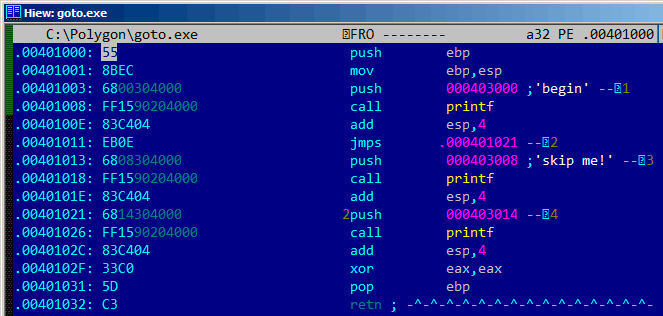
\includegraphics[scale=\FigScale]{patterns/065_GOTO/hiew1.png}
\caption{Hiew}
\label{fig:goto_hiew1}
\end{figure}

\clearpage
Поместите курсор по адресу \JMP (\TT{0x410}), 
нажмите F3 (редактирование), нажмите два нуля, так что
опкод становится \TT{EB 00}:

\begin{figure}[H]
\centering
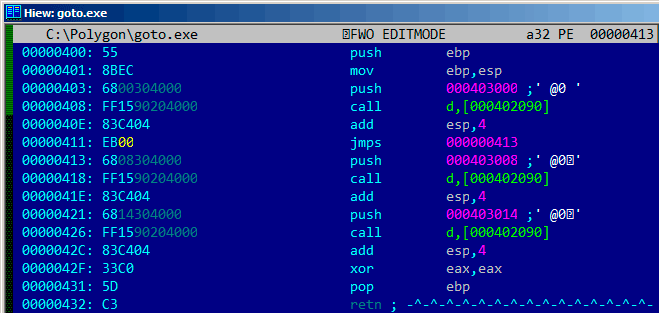
\includegraphics[scale=\FigScale]{patterns/065_GOTO/hiew2.png}
\caption{Hiew}
\label{fig:goto_hiew2}
\end{figure}

Второй байт опкода \JMP это относительное смещение от перехода. 0 означает место
прямо после текущей инструкции.
Теперь \JMP не будет пропускать следующий вызов \printf.
Нажмите F9 (запись) и выйдите.
Теперь мы запускаем исполняемый файл и видим это:

\begin{figure}[H]
\centering
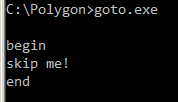
\includegraphics[scale=\NormalScale]{patterns/065_GOTO/result.png}
\caption{Результат}
\label{fig:goto_result}
\end{figure}

Подобного же эффекта можно достичь, если заменить инструкцию \JMP на две инструкции \NOP.
\NOP имеет опкод \TT{0x90} и длину в 1 байт, так что нужно 2 инструкции для замены.

\section{Мертвый код}

Вызов второго \printf также называется \q{мертвым кодом} (\q{dead code}) 
в терминах компиляторов.
Это значит, что он никогда не будет исполнен.
Так что если вы компилируете этот пример с оптимизацией, компилятор удаляет \q{мертвый
код} не оставляя следа:

\lstinputlisting[caption=\Optimizing MSVC 2012]{patterns/065_GOTO/MSVC_goto_Ox.asm}

Впрочем, строку \q{skip me!} компилятор убрать забыл.

%Note: cl "/Ox" option for maximum optimisation does get rid of "skip me" string as well

\section{\Exercise}

% TODO debugger example can fit here
Попробуйте добиться того же самого в вашем любимом компиляторе и отладчике.

